\documentclass[xetex,mathserif,serif]{beamer}
\usepackage{polyglossia}
\setdefaultlanguage[babelshorthands=true]{russian}
\usepackage{minted}
\usepackage{tabu}

\useoutertheme{infolines}

\usepackage{fontspec}
\setmainfont{FreeSans}
\newfontfamily{\russianfonttt}{FreeSans}

\setbeamertemplate{blocks}[rounded][shadow=false]
\setbeamercolor*{block title example}{fg=green!50!black,bg=green!20}
\setbeamercolor*{block body example}{fg=black,bg=green!10}

\setbeamercolor*{block title alerted}{fg=red!50!black,bg=red!20}
\setbeamercolor*{block body alerted}{fg=black,bg=red!10}

\tabulinesep=0.7mm

\title{Программирование на платформе .NET}
\subtitle{Введение, основы C\#}
\author[Юрий Литвинов]{Юрий Литвинов \newline \textcolor{gray}{\small\texttt{yurii.litvinov@gmail.com}}}

\date{1}

\begin{document}
	
	\frame{\titlepage}
	
	\begin{frame}
		\frametitle{О курсе}
		\begin{itemize}
			\item Рассказ про основные языки для .NET --- C\# и (немного) F\#
			\item Немного про саму платформу
			\item Будет также про основные библиотеки и технологии (WinForms, WPF, MVC, EF и т.д.)
			\item Лекции (каждую неделю), семинары (раз в несколько недель), домашние задания
			\item Оценка: домашние задания (70\%), экзамен в конце курса (30\%)
		\end{itemize}
	\end{frame}

	\begin{frame}
		\frametitle{Язык C\#}
		\begin{itemize}
			\item Объектно-ориентированный язык общего назначения с сильной типизацией
			\item Основной язык программирования для платформы .NET
			\item Первая версия --- 2002 год, актуальная --- 7.03.2017, C\# 7.0
			\item Международный стандарт (ISO/IEC 23270:2006)
			\item В основном для прикладного ПО
			\item 5-е место в индексе TIOBE
			\item Работает под Windows (.NET, .NET Core) и Linux/Mac OS (Mono, .NET Core)
			\item Средства разработки:
			\begin{itemize}
				\item Rider (\url{https://www.jetbrains.com/rider/})
				\item Microsoft Visual Studio (\url{https://www.visualstudio.com})
				\item MonoDevelop (\url{http://www.monodevelop.com/})
				\item Visual Studio Code (\url{https://code.visualstudio.com/})
			\end{itemize}
		\end{itemize}
	\end{frame}

	\begin{frame}
		\frametitle{Common Language Infrastructure}
		\begin{columns}
			\begin{column}{0.5\textwidth}
				\begin{small}
					\begin{itemize}
						\item Компиляция в байткод виртуальной машины (Common Intermediate Language, CIL)
						\item Виртуальная машина и набор библиотек (Common Language Runtime) реализуется для каждой платформы (ОС)
						%TODO: уточнить
						\item Машина интерпретирует байт-код или компилирует его <<на лету>> в машинные коды
						%TODO: найти ссылку с подтверждением
						\item Прежде всего для облегчения разработки компиляторов и обеспечения взаимодействия языков
					\end{itemize}
				\end{small}
			\end{column}
			\begin{column}{0.5\textwidth}
				\begin{center}
					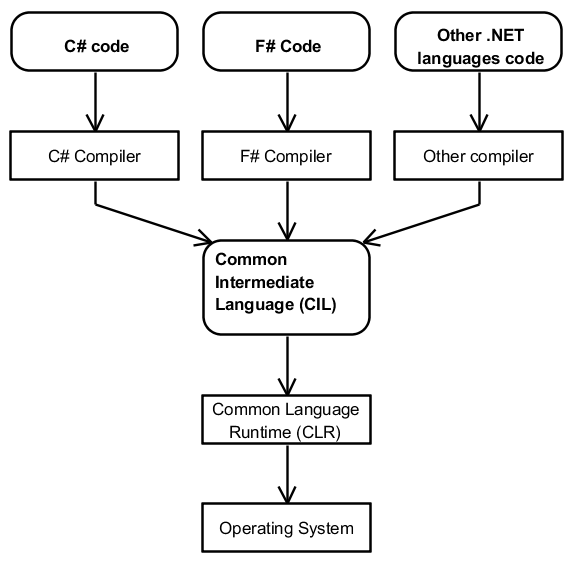
\includegraphics[width=\textwidth]{CLI.png}
				\end{center}
			\end{column}
		\end{columns}
	\end{frame}

	\begin{frame}[fragile]
		\frametitle{Технические подробности C\#}
		\framesubtitle{Как обычно, Hello, World}
		\begin{minted}{csharp}
using System;

namespace HelloWorld
{
    class Program
    {
        static void Main(string[] args)
        {
            Console.WriteLine("Goodbye, cruel world!");
        }
    }
}
		\end{minted}
\end{frame}

	\begin{frame}[fragile]
		\frametitle{Циклы}
		\begin{minted}{csharp}
for (int i = 0; i < 300; ++i)
{
    Console.WriteLine("Hello, world!");
}
		\end{minted}
		или
		\begin{minted}{csharp}
for (var i = 0; i < 300; ++i)
{
    Console.WriteLine("Hello, world!");
}
		\end{minted}
\end{frame}

	\begin{frame}[fragile]
		\frametitle{Методы}
		\begin{minted}{csharp}
private static int Factorial(int n)
{
    if (n <= 1)
    {
         return 1;
    }

    return n * Factorial(n - 1);
}
		\end{minted}
		или так:
		\begin{minted}{csharp}
private static int Factorial(int n) 
    => n <= 1 ? 1 : n * Factorial(n - 1);
		\end{minted}
\end{frame}

	\begin{frame}
		
	\end{frame}

\end{document}

